\documentclass[TQFT_main]{subfiles}

\begin{document}

% \setcounter{}{}

\chapter{粒子の統計性}

この章は~\cite[Chapter3, 4]{Simon2021}に相当する.この章では同種の多粒子系の経路積分による量子化を考察し,粒子の統計性と配位空間のホモトピー論の間の関係性を調べる.
特に,プロパゲーターの合成則を充たす経路積分の測度と配位空間の基本群のユニタリ表現の対応を考察し,$2+1$ 次元の同種 $N$ 粒子系においてエニオンの統計性が生じ得ることを確かめる.
なお,本章ではまだ場の量子化は行わない.

\section{1粒子の経路積分}

$\mathbb{R}^D$ 内を運動する非相対論的1粒子の軌跡 $\bm{x}(t)$ を与える.
時刻 $\irm{t}{i}$ に $\irm{\bm{x}}{i}$ を出発し,時刻 $\irm{t}{f}$ に $\irm{\bm{x}}{f}$ に到達しているとする.

この系を量子力学的に捉えてみる.時刻 $\irm{t}{i}$ に状態 $\ket{\irm{\bm{x}}{i}}$ にあった系が時刻 $\irm{t}{f}$ に状態 $\ket{\irm{\bm{x}}{f}}$ にある遷移振幅は\textbf{プロパゲーター} (propagator) と呼ばれるが,それは系の時間発展を表すユニタリ演算子 $\hat{U}(\irm{t}{f},\, \irm{t}{i})$ を用いて
\begin{align}
    \label{eq:1-def-propagator}
    \bra{\irm{\bm{x}}{f}} \hat{U}(\irm{t}{f},\, \irm{t}{i}) \ket{\irm{\bm{x}}{i}}
\end{align}
と書かれる\footnote{状態ケット $\ket{\bm{x}}$ はSchr\"{o}dinger表示である.}.プロパゲーターが計算されると,系の波動関数 $\psi(\bm{x},\, t) \coloneqq \braket{\bm{x}}{\psi(t)}$ の時間発展が次のようにしてわかる:
\begin{align}
    \psi(\irm{\bm{x}}{f},\, \irm{t}{f}) 
    &= \braket{\irm{\bm{x}}{f}}{\psi(\irm{t}{f})} \\
    &= \mel{\irm{\bm{x}}{f}}{\hat{U}(\irm{t}{f},\, \irm{t}{i})}{\psi(\irm{t}{i})} \\
    &= \int_{\mathbb{R}^D} \dd[D]{\irm{\bm{x}}{i}} \bra{\irm{\bm{x}}{f}} \hat{U}(\irm{t}{f},\, \irm{t}{i}) \ket{\irm{\bm{x}}{i}} \braket{\irm{\bm{x}}{i}}{\psi(\irm{t}{i})} \\ 
    &= \int_{\mathbb{R}^D} \dd[D]{\irm{\bm{x}}{i}} \bra{\irm{\bm{x}}{f}} \hat{U}(\irm{t}{f},\, \irm{t}{i}) \ket{\irm{\bm{x}}{i}} \psi(\irm{\bm{x}}{i},\, \irm{t}{i})
\end{align}
従って,初期条件が与えられてかつ任意の時刻を繋ぐプロパゲーターが計算できれば系の時間発展が全てわかったことになる.
そしてFeynmanの\textbf{経路積分} (path integral) による量子化とは,今考えている系の\underline{古典的}作用 
\begin{align}
    S[\bm{x}(t)] = \int_{\irm{t}{i}}^{\irm{t}{f}} \dd{t} L [\bm{x}(t),\, \dot{\bm{x}} (t),\, t]
\end{align}
と,\underline{量子的}なプロパゲーター\eqref{eq:1-def-propagator}との間に
\begin{align}
    \label{eq:1-pathintegral}
    \bra{\irm{\bm{x}}{f}} \hat{U}(\irm{t}{f},\, \irm{t}{i}) \ket{\irm{\bm{x}}{i}} = \mathcal{N} \sum_{\bm{x} (t)\, \mathrm{s.t.}\, \bm{x} (\irm{t}{i}) = \irm{\bm{x}}{i},\, \bm{x} (\irm{t}{f}) = \irm{\bm{x}}{f}} e^{\iunit S[\bm{x}(t)] / \hbar}
\end{align}
の関係があることを主張するものである.

いま考えている系のハミルトニアンが
\begin{align}
    \hat{H} (\hat{\bm{p}},\, \hat{\bm{x}}) = \frac{\hat{\bm{p}}^2}{2m} + V(\hat{\bm{x}})
\end{align}
と書かれる場合に\eqref{eq:1-pathintegral}が成り立っていることを確認する.Schr\"{o}dinger方程式より時間発展演算子は
\begin{align}
    \hat{U}(\irm{t}{f},\, \irm{t}{i}) = e^{-\iunit \hat{H}(\irm{t}{f} - \irm{t}{i}) / \hbar} 
\end{align}
である.十分大きな $n$ に対して $\varepsilon \coloneqq (\irm{t}{f} - \irm{t}{i} )/n$ とおくとことで時間間隔 $[\irm{t}{i},\, \irm{t}{f}]$ を
\begin{align}
    [\irm{t}{i},\, \irm{t}{f}] = [\irm{t}{i},\, \irm{t}{i}+\varepsilon] \cup [\irm{t}{i}+\varepsilon,\, \irm{t}{i}+2\varepsilon] \cup \cdots \cup [\irm{t}{i}+(n-1)\varepsilon,\, \irm{t}{f}]
\end{align}
のように分割し,$t_k \coloneqq \irm{t}{i} + k\varepsilon\; (k = 0,\, 1,\, \dots,\, n)$ とおく\footnote{定義から $\irm{t}{i} = t_0,\, \irm{t}{f} = t_n$ である.}.このとき $\varepsilon$ は微小なので,$\forall \bm{x}_k \in \mathbb{R}^D$ に対して
\begin{align}
    \bra{\bm{x}_{k+1}} \hat{U}(t_{k+1},\, t_k) \ket{\bm{x}_k} &= \bra{\bm{x}_{k+1}} e^{-\iunit \hat{H} \varepsilon / \hbar} \ket{\bm{x}_k} \\
    &\approx \braket{\bm{x}_{k+1}}{\bm{x}_k} - \frac{\iunit \varepsilon}{\hbar} \mel{\bm{x}_{k+1}}{\hat{H}}{\bm{x}_k} \\
    &= \delta^D (\bm{x}_{k+1} - \bm{x}_k) - \frac{\iunit \varepsilon}{\hbar} \left( \bra{\bm{x}_{k+1}} \frac{\hat{\bm{p}}}{2m} \ket{\bm{x}_k} + V (\bm{x}_k) \delta^D (\bm{x}_{k+1} - \bm{x}_k) \right) \\
    &= \int \frac{\dd^D \bm{p}}{(2\pi)^D} e^{\iunit \bm{p} \vdot (\bm{x}_{k+1} - \bm{x}_k)/\hbar} \left( 1 - \frac{\iunit \varepsilon}{\hbar} H (\bm{p},\, \bm{x}_k)  \right)\\
    &\approx \int \frac{\dd^D \bm{p}}{(2\pi)^D} e^{\iunit \bm{p} \vdot (\bm{x}_{k+1} - \bm{x}_k)/\hbar} e^{-\iunit \varepsilon H (\bm{p},\, \bm{x}_k) / \hbar}
\end{align}
が成り立つ.ここに,4行目以降に登場する $H (\bm{p},\, \bm{x}_k)$ は演算子ではなくc数である.
従って\footnote{実は,\eqref{eq:1-path1}から次の行への移行は,厳密には単に記号的なものだと考えるべきである.というのも,$\bm{x}_k\; (k=1,\, \dots,\, n-1)$ はそれぞれ独立に $\mathbb{R}^D$ を動くので,$(\bm{x}_{k+1} - \bm{x}_k)/\varepsilon$ は発散しても良いのである.つまり,次の行の $\dot{\bm{x}} \coloneqq \lim_{\varepsilon \to 0} (\bm{x}_{k+1} - \bm{x}_k)/\varepsilon$ は単に記号としてこう書いているだけに過ぎない.この件に関しては~\cite[第1章, p.23]{Nakahara2018topo1}に言及がある.旧版には書いていないので注意.},
\begin{align}
    &\bra{\irm{\bm{x}}{f}} \hat{U}(\irm{t}{f},\, \irm{t}{i}) \ket{\irm{\bm{x}}{i}} 
    = \bra{\irm{\bm{x}}{f}} e^{-\iunit \hat{H}n\varepsilon /\hbar} \ket{\irm{\bm{x}}{i}} \\
    &= \lim_{n\to \infty}\int \left(\prod_{k=1}^{n-1} \dd[D]{\bm{x}_k} \right) \prod_{k=0}^{n-1} \bra{\bm{x}_{k+1}} e^{-\iunit \hat{H} \varepsilon / \hbar} \ket{\bm{x}_k} \\
    &= \lim_{n\to \infty}\int \left(\prod_{k=0}^{n-1}  \frac{\dd[D]{\bm{x}_k}\dd^D \bm{p}_k}{(2\pi)^D} \right) \exp\left\{ \frac{\iunit}{\hbar} \varepsilon \sum_{k=0}^{n-1} \left(\bm{p}_k \vdot \frac{\bm{x}_{k+1} - \bm{x}_k }{\varepsilon} - H (\bm{p}_k,\, \bm{x}_k) \right)  \right\}  \label{eq:1-path1} \\ 
    &= \lim_{n\to \infty}\int \left(\prod_{k=1}^{n-1}  \frac{\dd[D]{\bm{x}_k}\dd^D \bm{p}_k}{(2\pi)^D} \right) \exp\left\{ \frac{\iunit}{\hbar} \int_{\irm{t}{i}}^{\irm{t}{f}} \dd{t} \bigl(\bm{p} \vdot \dot{\bm{x}} - H (\bm{p},\, \bm{x}) \bigr)  \right\} \\
    &\eqqcolon \int [\dd[D]{\bm{x}} \dd[D]{\bm{p}}] \exp\left\{ \frac{\iunit}{\hbar} \int_{\irm{t}{i}}^{\irm{t}{f}} \dd{t} \bigl(\bm{p} \vdot \dot{\bm{x}} - H (\bm{p},\, \bm{x}) \bigr)  \right\}
\end{align}
ただし $\int [\dd[D]{\bm{x}} \dd[D]{\bm{p}}] \coloneqq \lim_{n\to \infty}\int \left(\prod_{k=1}^{n-1}  \frac{\dd[D]{\bm{x}_k}\dd^D \bm{p}_k}{(2\pi)^D} \right)$ は経路積分の測度である.ハミルトニアンの $\bm{p}$ 依存性は運動項のみなので,\eqref{eq:1-path1}において $\bm{p}_k$ 積分を先に実行することができる:
\begin{align}
    \bra{\irm{\bm{x}}{f}} \hat{U}(\irm{t}{f},\, \irm{t}{i}) \ket{\irm{\bm{x}}{i}} 
    &= \lim_{\substack{n\to \infty \\ \mathrm{i.e.}\; \varepsilon \to 0}}\int \left(\prod_{k=1}^{n-1}  \frac{\dd[D]{\bm{x}_k}\dd^D \bm{p}_k}{(2\pi)^D} \right) \\
    &\qquad \exp\left\{ \frac{\iunit}{\hbar} \varepsilon \sum_{k=0}^{n-1} \left(- \frac{1}{2m} \left( \bm{p}_k - m\frac{\bm{x}_{k+1} - \bm{x}_k}{\varepsilon} \right)^2 + \frac{m}{2} \left( \frac{\bm{x}_{k+1} - \bm{x}_k}{\varepsilon} \right)^2 - V(\bm{x}_k) \right)  \right\} \\ 
    &= \lim_{\substack{n\to \infty \\ \mathrm{i.e.}\; \varepsilon \to 0}}\int \left(\prod_{k=1}^{n-1}  \left(\frac{m\hbar}{2\pi \iunit \varepsilon}\right)^{D/2} \dd[D]{\bm{x}_k} \right) \exp\left\{ \frac{\iunit}{\hbar} \varepsilon \sum_{k=0}^{n-1} \left(\frac{m}{2} \left( \frac{\bm{x}_{k+1} - \bm{x}_k}{\varepsilon} \right)^2 - V(\bm{x}_k) \right)  \right\} \\
    &= \lim_{n\to \infty}\int \left(\prod_{k=1}^{n-1}  \left(\frac{m\hbar}{2\pi \iunit \varepsilon}\right)^{D/2} \dd[D]{\bm{x}_k} \right) \exp\left\{ \frac{\iunit}{\hbar} \int_{\irm{t}{i}}^{\irm{t}{f}} \dd{t} \left(\frac{m}{2} \dot{\bm{x}}^2 - V(\bm{x}) \right)  \right\} \\
    &\eqqcolon \int [\dd[D]{\bm{x}}] \exp \left\{ \frac{\iunit}{\hbar} \int_{\irm{t}{i}}^{\irm{t}{f}} \dd{t} L [\bm{x}(t),\, \dot{\bm{x}} (t)] \right\} 
\end{align}
これがまさに求めたい形\eqref{eq:1-pathintegral}である.

\section{2つの同種粒子}

次に,$D (\ge 2)$ 次元Euclid空間\footnote{つまり,空間のRiemann計量の成分は $\delta_{ij}$ であるとする.} $\mathbb{R}^D$ 内に2つの同種粒子が存在する量子系 $\mathcal{H}$ を考える.簡単のためこの節では粒子の内部自由度はないとする.
% すなわち,Hilbert空間 $\mathcal{H}$ の元は $(\mathbb{R}^D)^2$ の元と1対1対応する.

\subsection{粒子の配位}

この系における粒子の配位 (configuration) を記述する方法を考察しよう.
% 今からやることを数学的に述べると,\textbf{配位空間} (configuration space) と呼ばれる集合 $\mathcal{C}$ と,それに付随する写像 $\mathcal{C} \lto \mathcal{H}$ を上手く定義するということである.
いま,\textit{\textbf{coincidences}}と呼ばれる集合を
$\Delta \coloneqq \bigl\{ (\bm{x},\, \bm{x}) \bigm| \bm{x} \in \mathbb{R}^D\bigr\}$
で定義する.内部自由度がないという仮定により,勝手な1つの $(\bm{x}_1,\, \bm{x}_2) \in (\mathbb{R}^D)^2 \setminus \Delta$ に対応する $\mathcal{H}$ の元が一意に定まる.それを $\ket{\bm{x}_1,\, \bm{x}_2} \in \mathcal{H}$ と書こう\footnote{写像 $\ket{\,,\, } \colon (\mathbb{R}^D)^2 \lto \mathcal{H}$ は全単射ではある.}.
ここで,いわゆる粒子の不可弁別性により2つのケット $\ket{\bm{x}_1,\, \bm{x}_2},\, \ket{\bm{x}_2,\, \bm{x}_1}$ が同じ物理状態\footnote{すなわち,Hilbert空間の元としては $\gU{1}$ 位相がかかるという違いしかない.}を表していることに注意する.
このため,集合 $(\mathbb{R}^D)^2 \setminus \Delta$ の上の同値関係 $\sim$ を
\begin{align}
    \sim\; \DEF (\bm{x}_1,\, \bm{x}_2) \sim (\bm{x}_2,\, \bm{x}_1)
\end{align}
と定義し,\textbf{配位空間} (configuration space) $\mathcal{C}$ としては\footnote{写像 $\mathcal{C} \lto \mathcal{H},\; [(\bm{x}_1,\, \bm{x}_2)] \lmto \ket{\bm{x}_1,\, \bm{x}_2}$ は代表元の取り方に依存するのでwell-definedでないが,この写像は $\mathcal{C}$ からHilbert空間 $\mathcal{H}$ の\textbf{射線} (ray) 全体が成す集合への写像だと思うことでwell-definedな全単射になる.$\mathcal{C}$ のことを配位空間と呼ぶのはこのためだと思われる.}商集合 $\bigl((\mathbb{R}^D)^2 \setminus \Delta\bigr) \bigm/ {\sim}$ を選ぶのが良い\footnote{というよりも実は,位相幾何学においては位相空間 $\mathcal{C}$ のことを $\mathbb{R}^D$ の $2$ 次の\textbf{(unordered) configuration space}と呼ぶ(\url{https://en.wikipedia.org/wiki/Configuration_space_(mathematics)}).$\mathbb{R}^D$ を一般の位相空間に置き換えても良い.}.

\begin{marker}
    以降では,同値類\footnote{$(\bm{x}_1,\, \bm{x}_2) \in (\mathbb{R}^D)^2 \setminus \Delta$ の $\sim$ による同値類を $[(\bm{x}_1,\, \bm{x}_2)]$ と書く.} $[(\bm{x}_1,\, \bm{x}_2)] \in \mathcal{C}$ の代表元として
    \begin{align}
        &y_1{}^1 < y_2{}^1 \\ 
        \OR \quad&y_1{}^1 = y_2{}^1,\, y_1{}^2 < y_2{}^2 \\
        \OR \quad&\cdots \\
        \OR \quad&y_1{}^1 = y_2{}^1,\, \cdots y_1{}^{D-1} = y_2{}^{D-1},\, y_1{}^D < y_2{}^D
    \end{align}
    を充たす $(\bm{y}_1,\, \bm{y}_2) \in [(\bm{x}_1,\, \bm{x}_2)]$ を使う.
\end{marker}

% 写像
% \begin{align}
%     \ket{\, ,\, } \colon \bigl((\mathbb{R}^D)^2 \setminus \Delta\bigr) \bigm/ {\sim} &\lto \mathcal{H} \\
%     [(\bm{x}_1,\, \bm{x}_2)] &\lmto \ket{(\bm{x}_1,\, \bm{x}_2)} \eqqcolon \ket{\bm{x}_1,\, \bm{x}_2}
% \end{align}
% を使う.ただし,$(\bm{x}_1,\, \bm{x}_2) \in (\mathbb{R}^D)^2 \setminus \Delta$ の $\sim$ による同値類を $[(\bm{x}_1,\, \bm{x}_2)]$ と書いた.
% 「粒子 $i\; (i = 1,\, 2)$ がそれぞれ位置 $\bm{x}_i \in \mathbb{R}^D$ にある」といった表現が意味をなさず,「位置 $\bm{x}_1 \in \mathbb{R}^D$ と $\bm{x}_2 \in \mathbb{R}^D$ の両方に粒子が存在する」と言うしかないこと,


\subsection{配位空間上の経路}

この系を経路積分によって量子化する際,積分すべき経路とは配位空間 $\mathcal{C}$ 上の連続曲線,すなわち連続写像 $l \colon [\irm{t}{i},\, \irm{t}{f}] \lto \mathcal{C}$ のことである.始点 $l(\irm{t}{i}) = [(\bm{x}_1{}_{\mathrm{i}},\, \bm{x}_2{}_{\mathrm{i}})] \eqqcolon \irm{\bm{x}}{i}$ および終点 $l(\irm{t}{f}) = [(\bm{x}_1{}_{\mathrm{f}},\, \bm{x}_2{}_{\mathrm{f}})] \eqqcolon \irm{\bm{x}}{f}$ を固定した経路全体がなすホモトピー集合を $\Pi \mathcal{C} (\irm{\bm{x}}{i},\, \irm{\bm{x}}{f})$ と書こう.
% この $\Pi \mathcal{C} (\irm{\bm{x}}{i},\, \irm{\bm{x}}{f})$ が\textbf{亜群} (groupoid) の構造を持つ
$\forall \bm{x}_{\mathrm{i}},\, \irm{\bm{x}}{m},\, \bm{x}_{\mathrm{f}} \in \mathcal{C}$ に対して,$\irm{\bm{x}}{i}$ と $\irm{\bm{x}}{m}$ を繋ぐ経路 $l_0$ と $\irm{\bm{x}}{m}$ と $\irm{\bm{x}}{f}$ を繋ぐ経路 $l_1$ の\textbf{積}と呼ばれる $\irm{\bm{x}}{i}$ と $\irm{\bm{x}}{f}$ を繋ぐ経路 $l_1 \cdot l_0$ を
\begin{align}
    (l_1 \cdot l_0)(t) \coloneqq 
    \begin{cases}
        l_0(2t - \irm{t}{i}), &t \in [\irm{t}{i},\, \frac{\irm{t}{i} + \irm{t}{f}}{2}] \\
        l_1(2t - \irm{t}{f}), &t \in [\frac{\irm{t}{i} + \irm{t}{f}}{2},\, \irm{t}{f}]
    \end{cases}
\end{align}
と定義し,$\irm{\bm{x}}{f}$ から $\irm{\bm{x}}{i}$ へむかう\textbf{逆}の経路を
\begin{align}
    (l^{-1})(t) \coloneqq l(\irm{t}{i} + \irm{t}{f} - t)
\end{align}
と定義する.
このとき,\underline{ホモトピー類の} well-defined な積が
\begin{align}
    * \colon \Pi \mathcal{C}(\irm{\bm{x}}{{m}},\, \irm{\bm{x}}{{f}}) \times  \Pi \mathcal{C}(\irm{\bm{x}}{{i}},\, \irm{\bm{x}}{{m}}) &\lto  \Pi \mathcal{C}(\irm{\bm{x}}{{i}},\, \irm{\bm{x}}{{f}}), \\
    ([l_1],\, [l_0]) &\lmto [l_1 \cdot l_0] \label{eq:1-pathprod}
\end{align}
と定義され,以下の性質を充たす.

\begin{mylem}[label=lem:1-1groupoid]{}
    $\forall \irm{\bm{x}}{i},\, \irm{\bm{x}}{m},\, \irm{\bm{x}}{n},\, \irm{\bm{x}}{f} \in \mathcal{C}$ に対して以下が成り立つ:
    \begin{enumerate}
        \item $\forall [l_0]\in \Pi \mathcal{C} (\irm{\bm{x}}{i},\, \irm{\bm{x}}{m}),\; \forall [l_1] \in \Pi \mathcal{C} (\irm{\bm{x}}{m},\, \irm{\bm{x}}{n}),\; \forall [l_2] \in \Pi \mathcal{C} (\irm{\bm{x}}{n},\, \irm{\bm{x}}{f})$ に対して
        \begin{align}
            ([l_2] * [l_1]) * [l_0] = [l_2] * ([l_1] * [l_0])
        \end{align}
        \item 定数写像 $[\irm{t}{i},\, \irm{t}{f}] \lto \mathcal{C},\; t \lmto \bm{x}$ のホモトピー類を $\unity_{\bm{x}}$ と書くとき,$\forall [l] \in \Pi \mathcal{C} (\irm{\bm{x}}{i},\, \irm{\bm{x}}{f})$ に対して
        \begin{align}
            [l] * \unity_{\irm{\bm{x}}{i}} = \unity_{\irm{\bm{x}}{f}} * [l]
        \end{align}
        \item $\forall [l] \in \Pi \mathcal{C} (\irm{\bm{x}}{i},\, \irm{\bm{x}}{f})$ に対して
        \begin{align}
            [l^{-1}] * [l] = \unity_{\irm{\bm{x}}{i}},\quad [l] * [l^{-1}] = \unity_{\irm{\bm{x}}{f}}
        \end{align}
    \end{enumerate}
\end{mylem}
つまり,始点と終点がつながっていさえすれば,集合 $\Pi \mathcal{C} \coloneqq \bigcup_{\irm{\bm{x}}{{i}},\, \irm{\bm{x}}{{f}} \in \mathcal{C}}\Pi \mathcal{C}(\irm{\bm{x}}{{i}},\, \irm{\bm{x}}{{f}})$ は積 $*$ に関して群のように振る舞う\footnote{このような代数的構造を\hyperref[def:groupoid]{亜群} (groupoid) と呼ぶ.$\Pi \mathcal{C}$ は位相空間 $\mathcal{C}$ の\textbf{基本亜群} (fundamental groupoid) と呼ばれる.}.特に $\irm{\bm{x}}{i} = \irm{\bm{x}}{f} = \bm{x}$ のとき $\Pi \mathcal{C}(\irm{\bm{x}}{i},\, \irm{\bm{x}}{f})$ は\textbf{基本群} (fundamental group) または $1$ 次の\textbf{ホモトピー群}と呼ばれ,$\pi_1 (\mathcal{C},\, \bm{x})$ と書かれる.

\begin{mylem}[]{}
    基本群は群である.
\end{mylem}

\begin{proof}
    始点と終点が一致しているので,$\forall [l_0],\, [l_1] \in \pi_1 (\mathcal{C},\, \bm{x})$ に対して積 $[l_0] * [l_1]$ が定義されている.
\end{proof}

今考えている系に関して言えば,群 $\pi_1(\mathcal{C},\, \bm{x})$ の位数は $\forall \bm{x} \in \mathcal{C}$ に対して常に $2$ であり,$\mathbb{Z}_2$ と同型である.

\subsection{経路積分による量子化}

配位空間 $\mathcal{C}$ 上の始点と終点をそれぞれ $[(\bm{x}_1{}_{\mathrm{i}},\, \bm{x}_2{}_{\mathrm{i}})] \eqqcolon \irm{\bm{x}}{i},\; [(\bm{x}_1{}_{\mathrm{f}},\, \bm{x}_2{}_{\mathrm{f}})] \eqqcolon \irm{\bm{x}}{f}$ に固定する.時刻 $\irm{t}{i}$ から $\irm{t}{f}$ までの系の時間発展演算子を $\hat{U}(\irm{t}{f},\,\irm{t}{i})$ と書くと,プロパゲーターは素朴に
\begin{align}
    \label{eq:1-propagator}
    &\bra{\bm{x}_1{}_{\mathrm{f}},\, \bm{x}_2{}_{\mathrm{f}}} \hat{U}(\irm{t}{f},\, \irm{t}{i}) \ket{\bm{x}_1{}_{\mathrm{i}},\, \bm{x}_2{}_{\mathrm{i}}} = \mathcal{N} \sum_{l \in \{\, \mathrm{ct.\,maps}\, [\irm{t}{i},\, \irm{t}{f}] \to \mathcal{C}\, \}} e^{\iunit S[l]/\hbar} \\
    &= \mathcal{N} \left( \sum_{l\, \ST [l] = +1} + \sum_{l\, \ST [l] = -1} \right) e^{\iunit S[l]/\hbar} \label{eq:1-propagator-b}
\end{align}
と計算される.これは以下の2つの性質を充たさねばならない:
\begin{enumerate}
    \item $\hat{U}(\irm{t}{f},\, \irm{t}{i})$ はユニタリ演算子
    \item 時刻 $\forall \irm{t}{m} \in [\irm{t}{i},\, \irm{t}{f}]$ に対して,
    \begin{align}
        \label{eq:1-composition}
        \bra{\bm{x}_1{}_{\mathrm{f}},\, \bm{x}_2{}_{\mathrm{f}}} \hat{U}(\irm{t}{f},\, \irm{t}{i}) \ket{\bm{x}_1{}_{\mathrm{i}},\, \bm{x}_2{}_{\mathrm{i}}} = \int \dd{\irm{\bm{x}_1}{m}}\dd{\irm{\bm{x}_2}{m}} \bra{\bm{x}_1{}_{\mathrm{f}},\, \bm{x}_2{}_{\mathrm{f}}} \hat{U}(\irm{t}{f},\, \irm{t}{m}) \ket{\bm{x}_1{}_{\mathrm{m}},\, \bm{x}_2{}_{\mathrm{m}}} \bra{\bm{x}_1{}_{\mathrm{m}},\, \bm{x}_2{}_{\mathrm{m}}} \hat{U}(\irm{t}{m},\, \irm{t}{i}) \ket{\bm{x}_1{}_{\mathrm{i}},\, \bm{x}_2{}_{\mathrm{i}}}
    \end{align}
\end{enumerate}
逆に (1), (2) を充たすような\eqref{eq:1-propagator}の最右辺には他の可能性がある.それは例えば
\begin{align}
    &\bra{\bm{x}_1{}_{\mathrm{f}},\, \bm{x}_2{}_{\mathrm{f}}} \hat{U}(\irm{t}{f},\, \irm{t}{i}) \ket{\bm{x}_1{}_{\mathrm{i}},\, \bm{x}_2{}_{\mathrm{i}}}\\
    &= \mathcal{N} \left( \sum_{l\, \ST [l] = +1} - \sum_{l\, \ST [l] = -1} \right) e^{\iunit S[l]/\hbar} \label{eq:1-propagator-f}
\end{align}
である.というのも,このとき $\Pi\mathcal{C}$ の積の性質(補題\ref{lem:1-1groupoid})および $\mathbb{Z}_2$ との類似から
\begin{align}
    &\int \dd{\irm{\bm{x}_1}{m}}\dd{\irm{\bm{x}_2}{m}} \bra{\bm{x}_1{}_{\mathrm{f}},\, \bm{x}_2{}_{\mathrm{f}}} \hat{U}(\irm{t}{f},\, \irm{t}{m}) \ket{\bm{x}_1{}_{\mathrm{m}},\, \bm{x}_2{}_{\mathrm{m}}} \bra{\bm{x}_1{}_{\mathrm{m}},\, \bm{x}_2{}_{\mathrm{m}}} \hat{U}(\irm{t}{m},\, \irm{t}{i}) \ket{\bm{x}_1{}_{\mathrm{i}},\, \bm{x}_2{}_{\mathrm{i}}} \\
    &\propto \int \dd{\irm{\bm{x}_1}{m}}\dd{\irm{\bm{x}_2}{m}} \left( \sum_{l_{\mathrm{m} \to \mathrm{f}}\, \ST [l_{\mathrm{m} \to \mathrm{f}}] = +1} - \sum_{l_{\mathrm{m} \to \mathrm{f}}\, \ST [l_{\mathrm{m} \to \mathrm{f}}] = -1} \right) e^{\iunit S[l_{\mathrm{m} \to \mathrm{f}}]/\hbar} \left( \sum_{l_{\mathrm{i} \to \mathrm{m}}\, \ST [l_{\mathrm{i} \to \mathrm{m}}] = +1} - \sum_{l_{\mathrm{i} \to \mathrm{m}}\, \ST [l_{\mathrm{i} \to \mathrm{m}}] = -1} \right) e^{\iunit S[l_{\mathrm{i} \to \mathrm{m}}]/\hbar} \\
    &= 
    \int \dd{\irm{\bm{x}_1}{m}}\dd{\irm{\bm{x}_2}{m}} \left( \sum_{[l_{\mathrm{m} \to \mathrm{f}}] = +1} \sum_{[l_{\mathrm{i} \to \mathrm{m}}] = +1} e^{\iunit (S[l_{\mathrm{m} \to \mathrm{f}}] + S[l_{\mathrm{i} \to \mathrm{m}}]) / \hbar} + \sum_{[l_{\mathrm{m} \to \mathrm{f}}] = -1} \sum_{[l_{\mathrm{i} \to \mathrm{m}}] = -1} e^{\iunit (S[l_{\mathrm{m} \to \mathrm{f}}] + S[l_{\mathrm{i} \to \mathrm{m}}])/\hbar}\right)  \\
    &\quad -\int \dd{\irm{\bm{x}_1}{m}}\dd{\irm{\bm{x}_2}{m}} \left( \sum_{[l_{\mathrm{m} \to \mathrm{f}}] = +1} \sum_{[l_{\mathrm{i} \to \mathrm{m}}] = -1} e^{\iunit (S[l_{\mathrm{m} \to \mathrm{f}}] + S[l_{\mathrm{i} \to \mathrm{m}}]) / \hbar} + \sum_{[l_{\mathrm{m} \to \mathrm{f}}] = -1} \sum_{[l_{\mathrm{i} \to \mathrm{m}}] = +1} e^{\iunit (S[l_{\mathrm{m} \to \mathrm{f}}] + S[l_{\mathrm{i} \to \mathrm{m}}])/\hbar}\right)  \\
    &=
    \int \dd{\irm{\bm{x}_1}{m}}\dd{\irm{\bm{x}_2}{m}} \sum_{[l_{\mathrm{m} \to \mathrm{f}} \cdot l_{\mathrm{i} \to \mathrm{m}}] = +1} e^{\iunit S[l_{\mathrm{m} \to \mathrm{f}} \cdot l_{\mathrm{i} \to \mathrm{m}}]/\hbar}
    -\int \dd{\irm{\bm{x}_1}{m}}\dd{\irm{\bm{x}_2}{m}} \sum_{[l_{\mathrm{m} \to \mathrm{f}} \cdot l_{\mathrm{i} \to \mathrm{m}}] = -1}e^{\iunit S[l_{\mathrm{m} \to \mathrm{f}} \cdot l_{\mathrm{i} \to \mathrm{m}}] / \hbar} \\
    &= \left( \sum_{l_{\mathrm{i} \to \mathrm{f}}\, \ST [l_{\mathrm{i} \to \mathrm{f}}] = +1} - \sum_{l_{\mathrm{i} \to \mathrm{f}}\, \ST [l_{\mathrm{i} \to \mathrm{f}}] = -1} \right) e^{\iunit S[l_{\mathrm{i} \to \mathrm{f}}]/\hbar}
    % \left( \sum_{l_{\mathrm{i} \to \mathrm{m}}\, \ST [l_{\mathrm{i} \to \mathrm{m}}] = +1} - \sum_{l_{\mathrm{i} \to \mathrm{m}}\, \ST [l_{\mathrm{i} \to \mathrm{m}}] = -1} \right) e^{\iunit S[l_{\mathrm{i} \to \mathrm{m}}]/\hbar} 
\end{align}
が成り立ち (2) が充たされるのである.ただし,2つめの等号で $S[l_{\mathrm{m} \to \mathrm{f}}] + S[l_{\mathrm{i} \to \mathrm{m}}] = S[l_{\mathrm{m} \to \mathrm{f}} \cdot l_{\mathrm{i} \to \mathrm{m}}]$ を使った.
\eqref{eq:1-propagator-f}はフェルミオンの経路積分を表す.

\section{同種粒子多体系}

次に $D (\ge 2)$ 次元Euclid空間 $\mathbb{R}^D$ 内に $N$ 個の同種粒子が存在する量子系 $\mathcal{H}$ を考える.簡単のためこの節でも粒子の内部自由度はないとし,粒子の生成・消滅は考えない.

経路積分による量子化では,2粒子の場合と同様の議論ができる.まず配位空間 $\mathcal{C}$ は,集合 $(\mathbb{R}^D)^N \setminus \Delta$ の上の同値関係
\begin{align}
    \sim \DEF (\bm{x}_1,\, \bm{x}_2,\, \dots,\, \bm{x}_N) \sim (\bm{x}_{\sigma(1)},\, \bm{x}_{\sigma(2)},\, \dots,\, \bm{x}_{\sigma(N)}),\quad \forall \sigma \in \mathfrak{S}_N
\end{align}
による\footnote{$\mathfrak{S}_N$ は $N$ 次の対称群.従って一つの同値類は $N!$ 個の $(\mathbb{R}^D)^N \setminus \Delta$ の元からなる.$\mathfrak{S}_N$ の作用による軌道空間と見ても良い.}商集合 $\bigl( (\mathbb{R}^D)^N \setminus \Delta \bigr) \bigm/ {\sim}$ として定義される.
積分すべき経路のホモトピー類は基本亜群 $\Pi \mathcal{C}$ をなす.
また,経路の世界線\footnote{つまり,$D+1$ 次元の粒子の軌跡.}を考えることでこれは $D + 1$ 次元空間を動く,互いに交わらない $N$ 本の曲線とみなすこともできる.
適当な基点 $\bm{x} \in (\mathbb{R}^D)^N \setminus \Delta$ を取ってきて基本群 $\pi_1 (\mathcal{C},\, \bm{x})$ を考えれば良い.
% 基本群 $\pi_1 (\mathcal{C},\, \bm{x})$ の構造がわかれば粒子の統計性が分かるはずである.


\subsection{$D = 2$ の場合:組み紐群}

空間次元が $D = 2$ の場合,$\pi_1 (\mathcal{C},\, \bm{x})$ は (Artinの) \textbf{組み紐群} (braid group) $B_N$ と呼ばれる.

\begin{mydef}[label=def:braidg]{組み紐群(代数的)}
    語 (word) $\{\sigma_1,\, \dots,\, \sigma_{N-1}\}$ で生成され,関係式
    \begin{align}
        \sigma_i \sigma_{i+1} \sigma_i &= \sigma_{i+1} \sigma_i \sigma_{i+1}& &1 \le i \le N - 2 \\ 
        \sigma_i \sigma_j &= \sigma_{j} \sigma_i  & &\abs{i-j} > 1,\; 1 \le i,\, j \le N - 1 \\ 
    \end{align}
    を充たす群を\textbf{Artinの組み紐群} (Artin braid group),もしくは単に\textbf{組み紐群} (braid group) と呼ぶ.
\end{mydef}

$B_N$ の代数的な定義\ref{def:braidg}と,位相幾何学的な定義 $\pi_1 (\mathcal{C},\, \bm{x})$ が同型であることは,例えば~\cite{Fadell1961braid}に証明がある.
生成元 $\sigma_i$ を図として表示することができる:
% \begin{figure}[H]
%     \centering
%     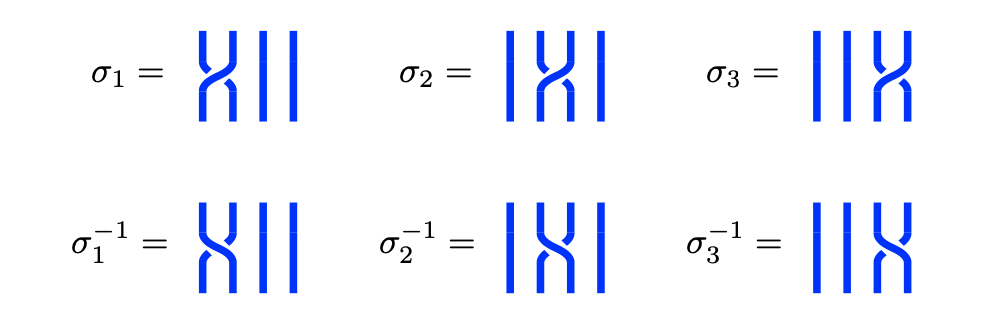
\includegraphics[scale=0.75]{./figs/braidg_generator.png}
%     \caption{$B_4$ の生成元の表示.~\cite[p.29, Fig. 3.4]{Simon2021}より引用.}
%     \label{fig:1-braidg-generator}
% \end{figure}%
\begin{align}
    \sigma_1 &\coloneqq
    \begin{tikzpicture}[baseline={([yshift=-.5ex]current bounding box.center)}]
        \path 
        foreach \x in {0,...,3} {
            foreach \y in {0,1} {
                coordinate (v_\x\y) at ({0.5*\x}, \y)
            }
        };
        \begin{knot}
            \strand[ultra thick] (v_00) .. controls +(0,0.7) and +(0,-0.7) .. (v_11);
            \strand[ultra thick] (v_10) .. controls +(0,0.7) and +(0,-0.7) .. (v_01);
        \end{knot}
        \draw[ultra thick] (v_20) -- (v_21);
        \draw[ultra thick] (v_30) -- (v_31);
    \end{tikzpicture}
    &
    \sigma_2 &\coloneqq
    \begin{tikzpicture}[baseline={([yshift=-.5ex]current bounding box.center)}]
        \path 
        foreach \x in {0,...,3} {
            foreach \y in {0,1} {
                coordinate (v_\x\y) at ({0.5*\x}, \y)
            }
        };
        \begin{knot}
            \strand[ultra thick] (v_10) .. controls +(0,0.7) and +(0,-0.7) .. (v_21);
            \strand[ultra thick] (v_20) .. controls +(0,0.7) and +(0,-0.7) .. (v_11);
        \end{knot}
        \draw[ultra thick] (v_00) -- (v_01);
        \draw[ultra thick] (v_30) -- (v_31);
    \end{tikzpicture}
    &
    \sigma_3 &\coloneqq
    \begin{tikzpicture}[baseline={([yshift=-.5ex]current bounding box.center)}]
        \path 
        foreach \x in {0,...,3} {
            foreach \y in {0,1} {
                coordinate (v_\x\y) at ({0.5*\x}, \y)
            }
        };
        \begin{knot}
            \strand[ultra thick] (v_20) .. controls +(0,0.7) and +(0,-0.7) .. (v_31);
            \strand[ultra thick] (v_30) .. controls +(0,0.7) and +(0,-0.7) .. (v_21);
        \end{knot}
        \draw[ultra thick] (v_00) -- (v_01);
        \draw[ultra thick] (v_10) -- (v_11);
    \end{tikzpicture} \\
    & \\
    \sigma_1^{-1} &\coloneqq
    \begin{tikzpicture}[baseline={([yshift=-.5ex]current bounding box.center)}]
        \path 
        foreach \x in {0,...,3} {
            foreach \y in {0,1} {
                coordinate (v_\x\y) at ({0.5*\x}, \y)
            }
        };
        \begin{knot}[flip crossing=1]
            \strand[ultra thick] (v_00) .. controls +(0,0.7) and +(0,-0.7) .. (v_11);
            \strand[ultra thick] (v_10) .. controls +(0,0.7) and +(0,-0.7) .. (v_01);
        \end{knot}
        \draw[ultra thick] (v_20) -- (v_21);
        \draw[ultra thick] (v_30) -- (v_31);
    \end{tikzpicture}
    &
    \sigma_2^{-1} &\coloneqq
    \begin{tikzpicture}[baseline={([yshift=-.5ex]current bounding box.center)}]
        \path 
        foreach \x in {0,...,3} {
            foreach \y in {0,1} {
                coordinate (v_\x\y) at ({0.5*\x}, \y)
            }
        };
        \begin{knot}[flip crossing=1]
            \strand[ultra thick] (v_10) .. controls +(0,0.7) and +(0,-0.7) .. (v_21);
            \strand[ultra thick] (v_20) .. controls +(0,0.7) and +(0,-0.7) .. (v_11);
        \end{knot}
        \draw[ultra thick] (v_00) -- (v_01);
        \draw[ultra thick] (v_30) -- (v_31);
    \end{tikzpicture}
    &
    \sigma_3^{-1} &\coloneqq
    \begin{tikzpicture}[baseline={([yshift=-.5ex]current bounding box.center)}]
        \path 
        foreach \x in {0,...,3} {
            foreach \y in {0,1} {
                coordinate (v_\x\y) at ({0.5*\x}, \y)
            }
        };
        \begin{knot}[flip crossing=1]
            \strand[ultra thick] (v_20) .. controls +(0,0.7) and +(0,-0.7) .. (v_31);
            \strand[ultra thick] (v_30) .. controls +(0,0.7) and +(0,-0.7) .. (v_21);
        \end{knot}
        \draw[ultra thick] (v_00) -- (v_01);
        \draw[ultra thick] (v_10) -- (v_11);
    \end{tikzpicture}
\end{align}
図において,$B_N$ の積とは単に組み紐を下から上へ\footnote{文献によって上下がまちまちである.}繋げることに他ならない.

組み紐不変量として特に重要なのが\textbf{巻き付き数} (winding number) である:
\begin{align}
    W \coloneqq (\#\, \text{of overcrossings}) - (\#\, \text{of undercrossings})
\end{align}

\subsection{$D = 3$ の場合:対称群}

空間次元が $D = 3$ の場合,$\pi_1 (\mathcal{C},\, \bm{x})$ の様子は $D=2$ の場合と大きく異なる.

\begin{myprop}[label=prop:not4D-knot]{}
    $S^1$ の $\mathbb{R}^3$ への任意の2つの\hyperref[def:submersion-smooth]{位相的埋め込み}は,それらを $\mathbb{R}^4$ への位相的埋め込み埋め込みと見做すことで互いにアイソトピックになる.
\end{myprop}

命題\ref{prop:not4D-knot}により,$D=3$ のとき $\pi_1 (\mathcal{C},\, \bm{x}) = \mathfrak{S}_N$ であることが分かる. 

\subsection{経路積分の構成}

$N = 2$ の場合と同様に考える.経路積分の終点と始点を $\{\bm{x}\}_{\mathrm{i}},\, \{\bm{x}\}_{\mathrm{f}} \in \mathcal{C}$ に固定する.
まず簡単のため $\{\bm{x}\}_{\mathrm{i}} = \{\bm{x}\}_{\mathrm{f}} \eqqcolon \{\bm{x}\}$ とすると,
\begin{align}
    \bra{\{\bm{x}\}_{\mathrm{f}}} \hat{U}(\irm{t}{f},\, \irm{t}{i}) \ket{\{\bm{x}\}_{\mathrm{i}}} =\mathcal{N} \sum_{[l] \in \pi_1(\mathcal{C},\, \{\bm{x}\})} \rho([l]) \sum_{m \in [l]} e^{\iunit S[m]/\hbar}
\end{align}
とすれば条件 \eqref{eq:1-composition} が充たされる.ただしユニタリ性の条件を充たすため,
% 群準同型
% \begin{align}
%     \rho \colon \pi_1(\mathcal{C},\, \{\bm{x}\}) \lto \Hom{\mathcal{H}}
% \end{align}
群準同型
$\rho \colon \pi_1(\mathcal{C},\, \{\bm{x}\}) \lto \mathrm{GL}(V)$ 
は基本群 $\pi_1(\mathcal{C},\, \{\bm{x}\})$ の\underline{ユニタリ表現}にとる.

\subsection{1次元表現(可換な例)}

まず $\rho$ が $\pi_1(\mathcal{C},\, \{\bm{x}\})$ の1次元ユニタリ表現である場合を考える.つまり,群準同型 $\rho \colon \pi_1(\mathcal{C},\, \{\bm{x}\}) \lto \gU{1}$ としてあり得るものを全て列挙することを試みる.

\begin{myexample}[label=ex:1-1abelian]{$2+1$ 次元の場合}
    $\pi_1(\mathcal{C},\, \{\bm{x}\}) = B_N$ である.$N-1$ 個の $\gU{1}$ の元の組 $\{g_1,\, \dots ,\, g_{N-1}\}$ であって定義\ref{def:braidg}の関係式を充たすものを見つければ良い.
    $\gU{1}$ は可換群なので2つ目の関係式は常に成り立つ.1つ目の関係式が成り立つ必要十分条件は $g_1 = g_2 = \cdots  = g_{N-1} = e^{\iunit \theta}$ ($\theta \in \mathbb{R}$ は任意)である.
    $1 \le \forall i \le N-1$ に対して $W(\sigma_i) = 1$ であることから,
    \begin{align}
        \rho_\theta (g) \coloneqq e^{\iunit \theta W(g)}\quad (\forall \theta \in \mathbb{R})
    \end{align}
    によって全ての表現が尽くされた.
    \begin{itemize}
        \item $\theta = 0$ のとき $\rho_\theta \colon g \lmto 1$ であり,\textbf{ボゾン}
        \item $\theta = \pi$ のとき $\rho_\theta \colon g \lmto (-1)^{W(g)}$ であり,\textbf{フェルミオン}
        \item 他の $\theta \in \mathbb{R}$ に対応する $\rho_\theta$ による統計性は\textbf{エニオン} (anyons),もしくは\textbf{分数統計} (fractional statistics) と呼ばれる.
        特に $\gU{1}$ が可換群なので\textbf{可換エニオン} (abelian anyons) という.
    \end{itemize}
\end{myexample}

\begin{myexample}[label=ex:1-2abelian]{$3+1$ 次元の場合}
    $\pi_1(\mathcal{C},\, \{\bm{x}\}) = \mathfrak{S}_N$ である.定義\ref{def:braidg}の関係式に $\sigma_i^2 = \unity$ を追加したものが $\mathfrak{S}_N$ のCoxeter presentationとなる.つまり,\exref{ex:1-1abelian}において $\theta = 0,\, \pi$ の場合のみがあり得る.これはボゾンとフェルミオンであり,$N=2$ の場合に考察した例の一般化になっている.
\end{myexample}

\subsection{より高次元の表現(非可換な場合)}

粒子の内部自由度を考慮しよう.具体的には,$D (\ge 2)$ 次元Euclid空間 $\mathbb{R}^D$ 内に $N$ 個の同種粒子が存在する量子系 $\mathcal{H}$ において内部自由度を指定する添字集合 $\mathcal{I}$ が存在して,写像
\begin{align}
    \ket{\, ;\, } \colon \bigl((\mathbb{R}^D)^N \setminus \Delta\bigr) \times \mathcal{I} \lto \mathcal{H},\; \bigl((\bm{x}),\, i\bigr) \lmto \ket{\{\bm{x}\};\, i}
\end{align}
が全単射となるような状況を考える\footnote{ややこしいが,定義域を同値関係で割る前なので $(\bm{x})$ と表記した.}.このとき $\forall \{\bm{x}\}_{\mathrm{i}},\, \{\bm{x}\}_{\mathrm{f}} \in \mathcal{C},\; \forall i,\, j \in \mathcal{I}$ に対するプロパゲーター
\begin{align}
    \bra{\{\bm{x}\}_{\mathrm{f}};\, i} \hat{U} (\irm{t}{f},\, \irm{t}{i}) \ket{\{\bm{x}\}_{\mathrm{i}};\, j} = \mathcal{N} \sum_{[l] \in \pi_1(\mathcal{C},\, \{\bm{x}\})} \bigl[\, \rho([l])\, \bigr]_{ij} \sum_{m \in [l]} e^{\iunit S[m]/\hbar}
\end{align}
を計算する必要がある.ここに,$\# \mathcal{I} = M < \infty$ のとき群準同型
\begin{align}
    \rho \colon \pi_1 (\mathcal{C},\, \{\bm{x}\}) \lto \gU{M} \subset \gGL{\mathbb{C}}{M}
\end{align}
は $\pi_1 (\mathcal{C},\, \{\bm{x}\})$ の $M$ 次元ユニタリ表現であり,$\bigl[\, \rho([l])\, \bigr]_{ij}$ というのは $M \times M$ ユニタリ行列 $\rho([l])$ の第 $(i,\, j)$ 成分という意味である.
一方 $\# \mathcal{I} = \infty$ のとき $\rho$ は無限次元表現となる.

\begin{myexample}[label=ex:1-3nonabelian]{$2+1$ 次元の場合}
    特に空間次元が $D=2$ のとき,$\rho$ は $B_N$ の $M$ 次元ユニタリ表現である.このような統計性を持つ粒子のことを\textbf{非可換エニオン} (nonabelian anyon) と呼ぶ\footnote{$\gU{M}$ が非可換群なので}.
\end{myexample}


\begin{myexample}[label=ex:1-3nonabelian]{$3+1$ 次元の場合}
    特に空間次元が $D=3$ のとき,$\rho$ は $\mathfrak{S}_N$ の $M$ 次元ユニタリ表現である.このような統計性を持つ粒子のことを\textbf{parastatistics}と呼ぶが,
    実は暗に存在する付加的な制約のせいでボゾンかフェルミオン,もしくはいくつか内部自由度が追加されるかしか許されないことが示されている~\cite[Appendix B]{HalvorsonMuger2006}.このことについては後述する.
    しかし,粒子の描像を捨てて弦を考えるなどすると「面白い」例が得られるかもしれない.
\end{myexample}




\end{document}